\documentclass[12pt, letterpaper]{article}
\usepackage[utf8]{inputenc}
\usepackage{natbib}
\usepackage{graphicx}
\usepackage{titlepic}
\usepackage{verbatim}
\usepackage{hyperref}

\hypersetup{
    colorlinks=true,
    linkcolor=black,
    filecolor=magenta,      
    urlcolor=blue,
    pdftitle = {Getting Started With Versaplanetary Gearboxes},
    bookmarks = true,}

\title{Getting Started With Versaplanetary Gearboxes}
\author{Nitzan Friedberg, FRC \#3928}
\date{}
\titlepic{
\includegraphics[width=\textwidth]{Logo-Dark Colors.png}}

\begin{document}

\maketitle

\tableofcontents

\newpage

\section{Introduction}
This is meant to be a guide to give people a starting point for using Vex Versaplanetary gearboxes. It is not meant to be comprehensive documentation, Vex has done a great job of including extensive documentation on their \href{https://www.vexrobotics.com/versaplanetary.html}{website}. 

\subsection{Background}
Versaplanetary gearboxes were developed by Vex Robotics in 2013  and have been very useful in FRC designs for their ability to have large reductions in a small package as well as the ability to quickly change gear ratio by swapping, adding, or removing stages. 

\begin{figure}[h!]
\centering
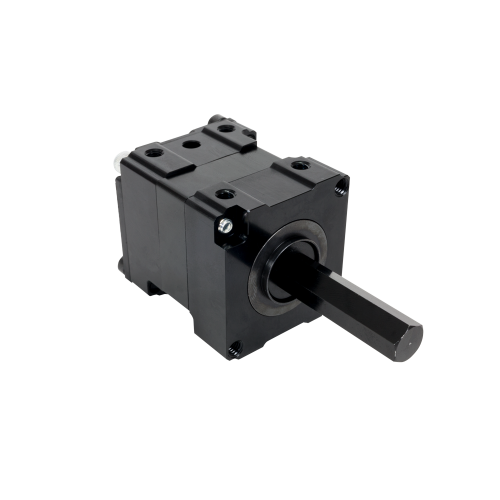
\includegraphics[scale=0.5]{Versaplanetary.png}
\caption{Versaplanetary Gearbox}
\label{fig:Versaplanetary Gearbox}
\end{figure}

\subsection{Planetary Gearboxes}
A planetary gearbox has 3 essential parts: a sun gear, planet gears, and a ring gear. This allows for a large reduction while taking up a small volume. A few drawbacks of of planetary gearboxes in FRC is that there is an efficiency loss of \~{}10\% per stage. Another drawback is that the small size of the teeth on planetary gears makes them more prone to breaking when compared to other spur gears  used in FRC.

\begin{figure}[h!]
    \centering
    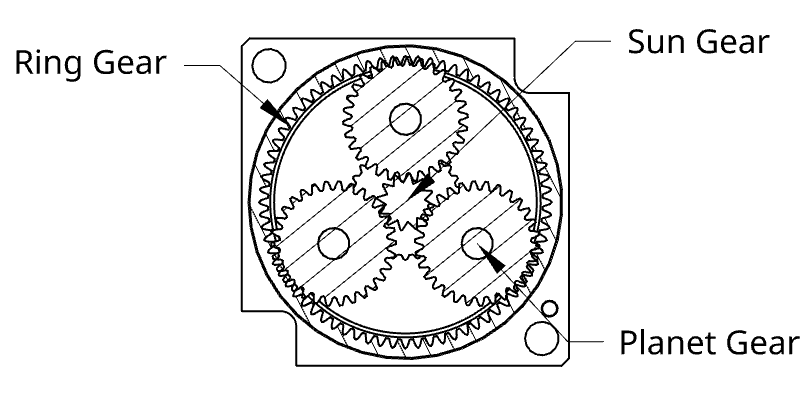
\includegraphics[scale=0.5]{Planetary Gearbox.png}
    \caption{Section view of a Versaplanetary gearbox}
    \label{fig:section view}
\end{figure}

\subsection{v1 vs. v2 Versaplanetaries}
In 2016 Vex released a second version of the Versaplanetary with  screws that are installed from the "back," which is makes  it much easier to swap motors without taking apart the entire gearbox. \textbf{The v1 \& v2 input and output blocks cannot be mixed and matched - A v2 input block must be used with a v2 output block. Ring gears and gear kits are compatible between v1 \& v2}

\begin{figure}[h!]
\centering
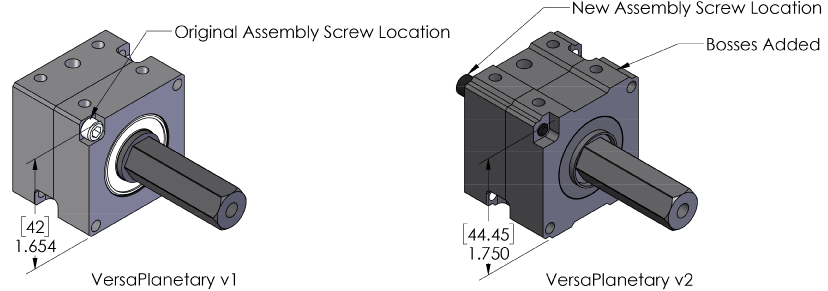
\includegraphics[scale = 0.625]{v1v2.png}
\caption{Comparison of v1 \& v2 gearboxes}
\label{fig:v1v2 Comparison}
\end{figure}

\section{Load Ratings}
When designing mechanisms that use Versaplanetaries, it is important to reference Vex's published load ratings to ensure that the reduction you are planning to use doesn't break under load. There are many different tables for various output shaft configurations, but the most common use case for Versaplanetaries is using a 1/2" hex output shaft.

In general, higher torque motors such as CIMs, NEOs, and Falcons cannot be run with high 2 stage reductions, while lower torque motors such as the BAG Motor or 775pro are within rating up to the maximum 2 stage reduction (100:1). Adding a 3rd stage can be useful, but there are much fewer configurations that are within load ratings.

\subsection{Additional reduction}
It can be useful to add an additional reduction to a Veraplanetary, for example, driving a chain and sprocket. This can be useful for: (1) reducing shock loads on the gearbox, and (2) reducing the necessary reduction within the Versaplanetary, allowing designs to be well within load ratings.

%\newpage
\section{Assembly}
Vex has great documentation on assembling Versaplanetaries in their \href{https://content.vexrobotics.com/vexpro/pdf/VersaPlanetary-v2-UserGuide-20170403.pdf}{user guide}, but there are a  few things that should be emphasized:
\begin{itemize}
    \item Order of stages in multi-stage gearboxes:
    \newline The higher reduction stage should be placed closer to the motor, higher reduction stages are easier to break and should be placed where they experience lower torque.
    
    \item  Matching carrier plates to gear sets:
    \newline Carrier plates are designed with specific spacing for their specific reduction. It is easy to mix up sun \& planet gears with the wrong carrier plate. Ensure that the gears in each stage are meshing properly.
    
    \item Motor shaft coupler assembly:
    \newline The  motor shaft coupler needs to be oriented correctly with the input coupler. It is also important to leave a small gap between the input coupler and the motor plate.

    \begin{figure}[h!]
        \centering
        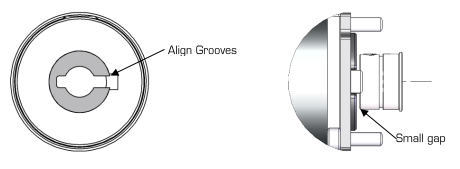
\includegraphics[scale = 0.5]{Shaft coupler.png}
        \caption{Shaft coupler assembly}
    \end{figure}
    
    \item Checking for jams:
    \newline Make sure to check the gearbox is free spinning before you power it. It might be necessary to use a 1/2" wrench to spin the gearbox if the reduction is large.
    
    \item Use grease!

\end{itemize}


\section{Known Problems}
\begin{itemize}
    \item 10:1 Stages:
    \newline The sun gears on 10:1 stages are extremely small and are easy to break, even when within load ratings. Only use 10:1 reductions for light load applications if possible. A 10:1 reduction on an intake roller would probably be fine, but using a 10:1 reduction on a higher reduction mechanism such as a large arm (where shock loads can be common) is generally a bad idea.

    \begin{figure}[h!]
        \centering
        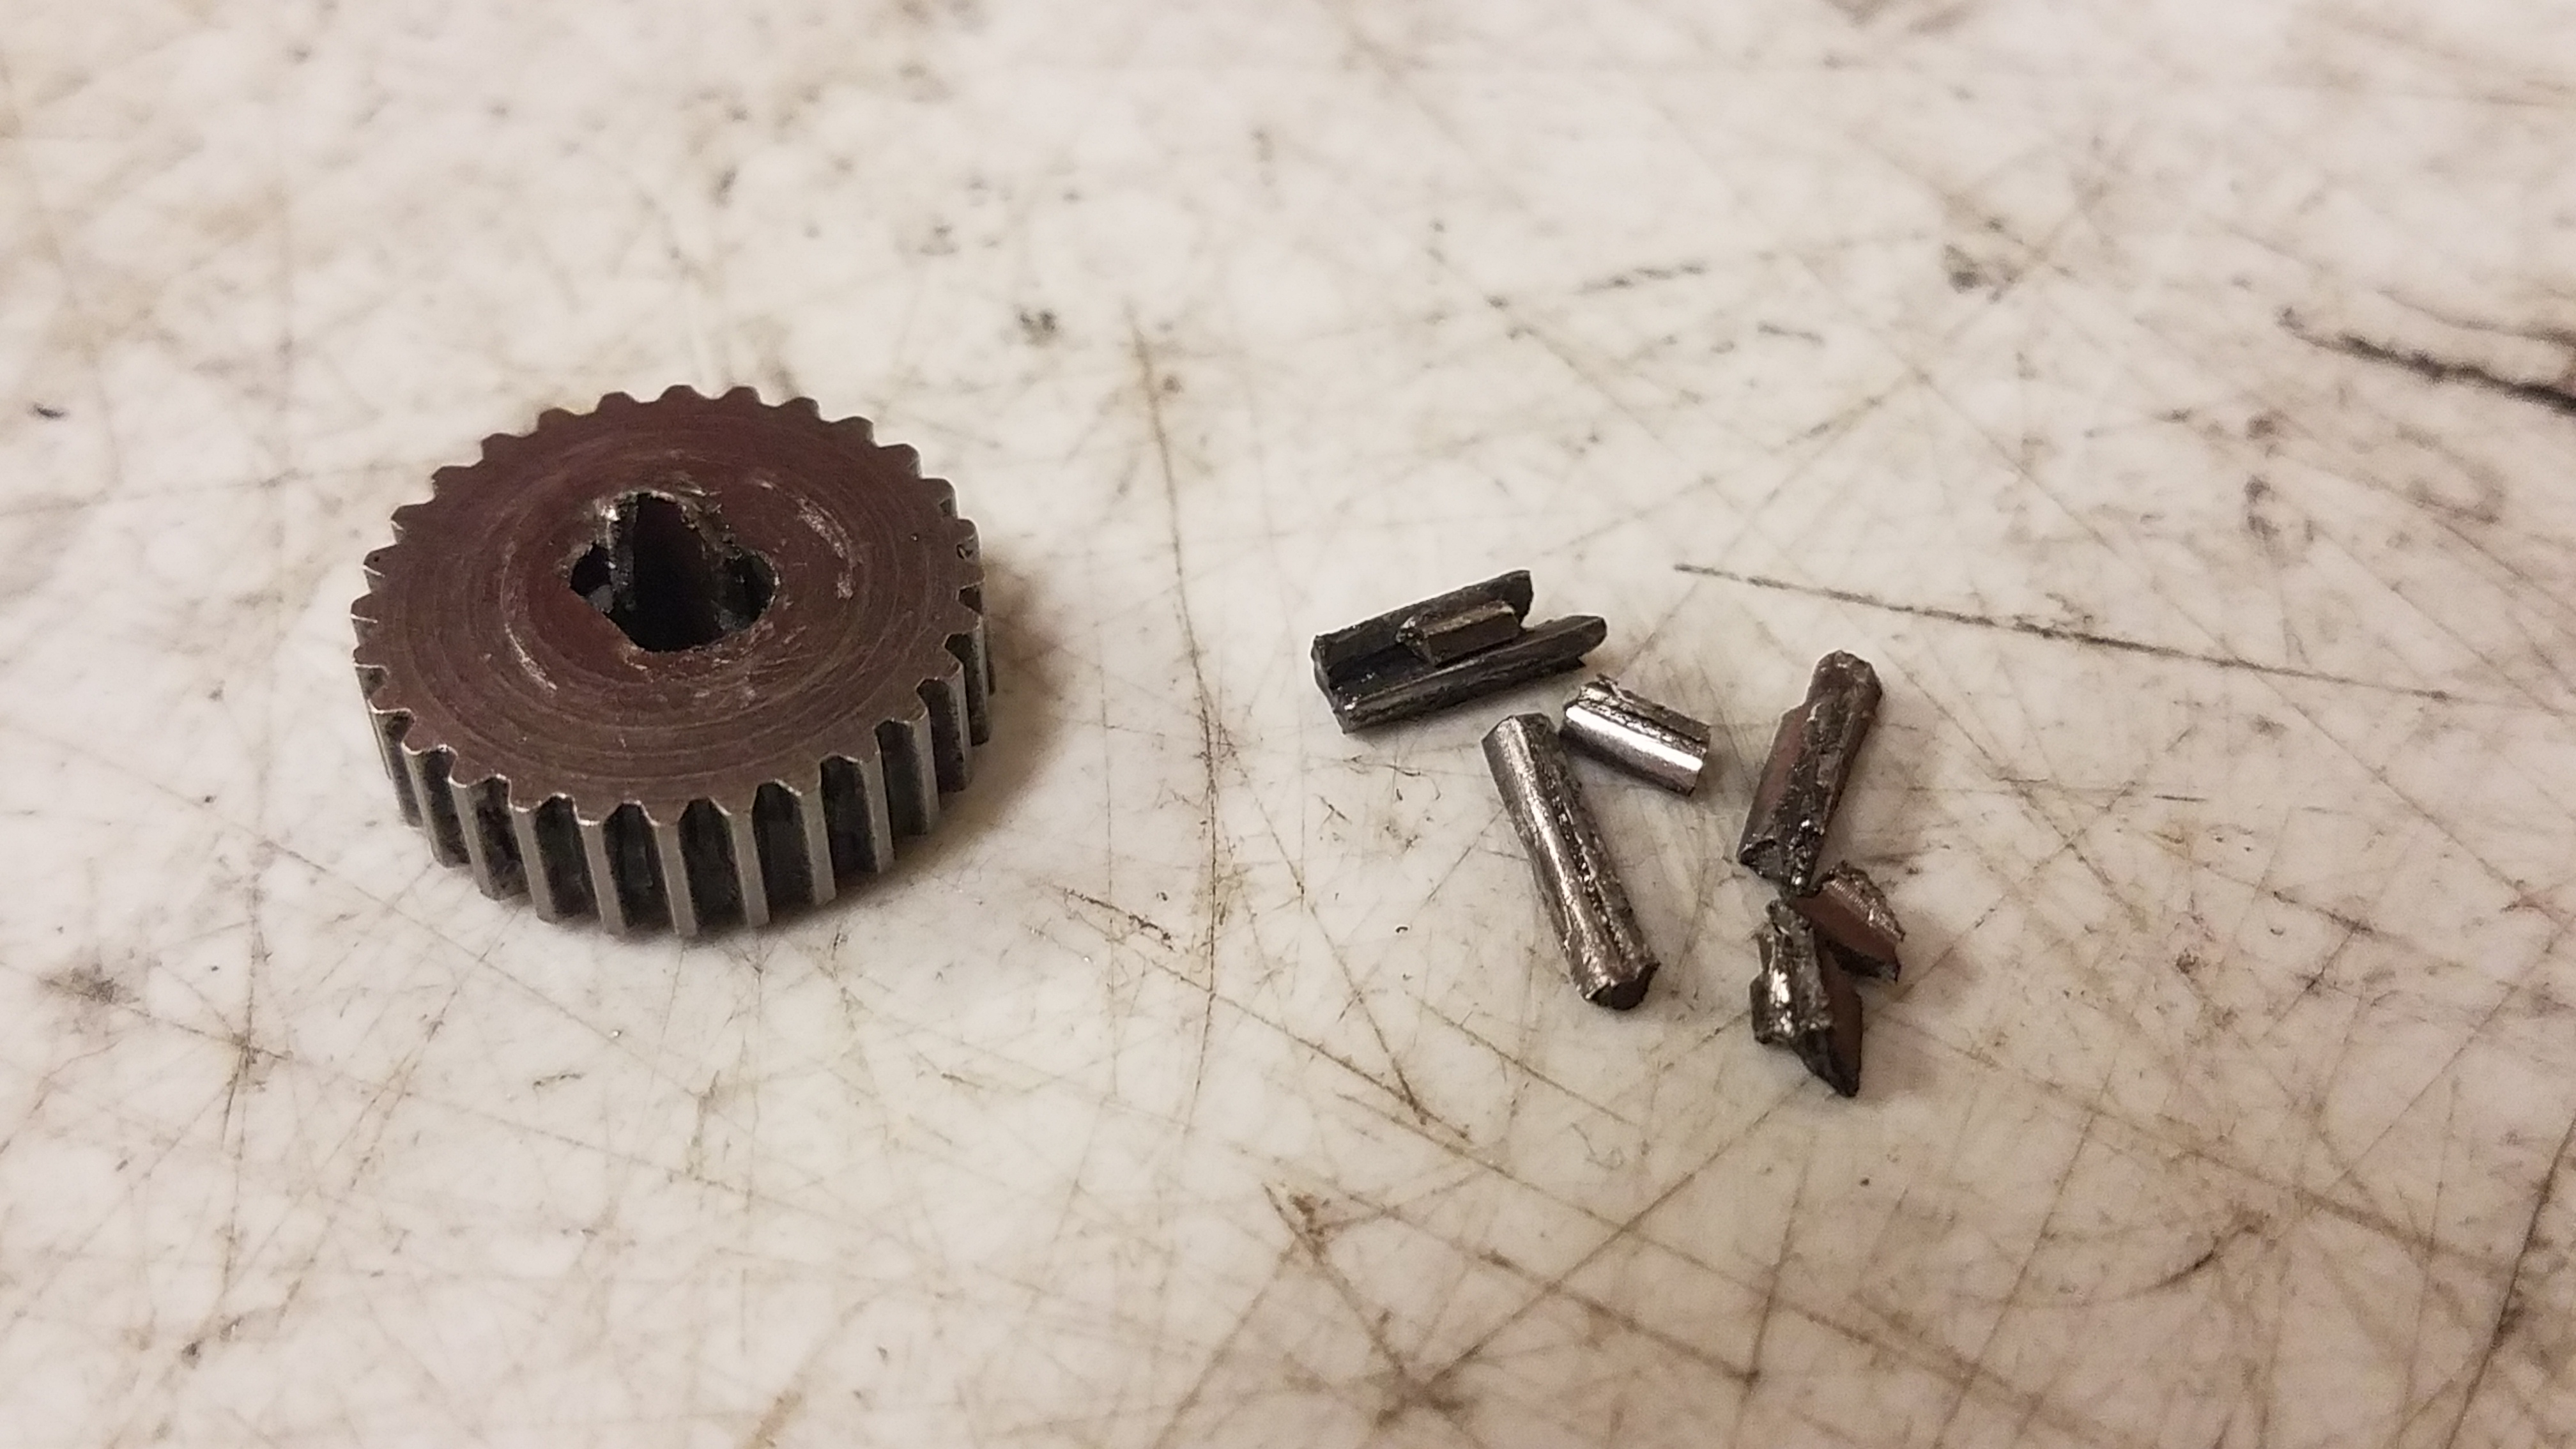
\includegraphics[scale = 0.0625]{broken versa 2.jpeg}
        \caption{Broken 10:1 sun gear}
    \end{figure}
    
    \item Output shaft snap ring groove wear: 
    \newline The area behind the snap ring groove on the output shaft can wear down allowing the snap ring that retains the shaft to move out of place. This can cause output shaft to lose engagement with the rest of the gearbox.

    \begin{figure}[h!]
        \centering
        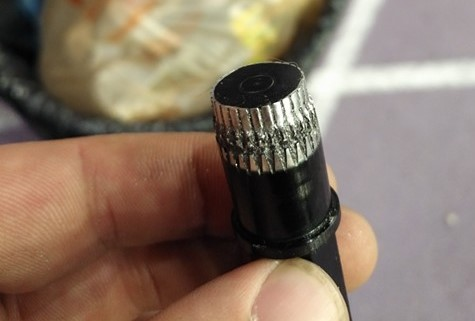
\includegraphics[scale = 0.5]{stripped output.jpeg}
        \caption{Extremely worn output shaft}
    \end{figure}

    \item Loose carrier plate pins:
    \newline If the pins in a carrier plate are not flush or are able to move around, they should be pressed into place and secured.

    \begin{figure}[h!]
        \centering
        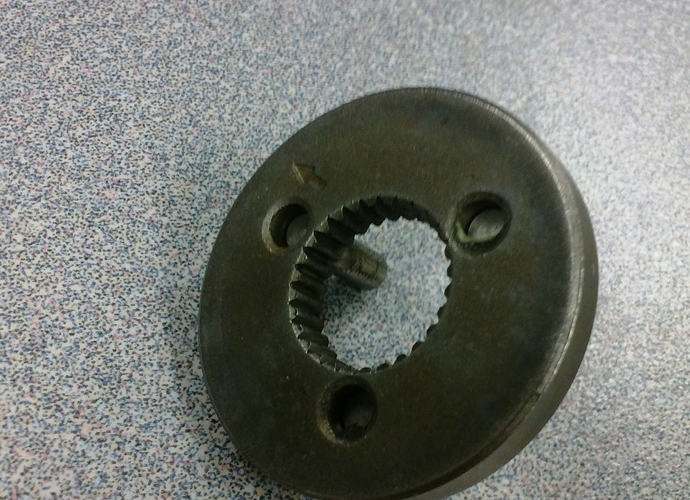
\includegraphics[scale = 0.35]{Carrier Plate.jpeg}
        \caption{Carrier plate with loose pins}
    \end{figure}


\end{itemize}

\begin{comment}

\section{Conclusion}
``I always thought something was fundamentally wrong with the universe'' \citep{adams1995hitchhiker}

\bibliographystyle{plain}
\bibliography{references}
\end{comment}
\end{document}